%!TEX root=betamain.tex


\section{Introduction}
\label{sec:intro}

Crowdsourcing provides an efficient method 
to annotate data on a large scale for various machine learning tasks, 
by employing a massive workforce drawn from global Internet users.
Popular online crowdsourcing platforms include
Amazon Mechanical Turk\footnote{\url{https://www.mturk.com/}} and CrowdFlower\footnote{\url{http://www.crowdflower.com/}}.
However, while crowdsourcing is relatively cheap compared
to employing experts, getting large quantities of labeled data
annotated by crowds (say thousands, or millions of data items) 
can be rather expensive. 
% However, in contrast to data annotated by experts,
% crowdsourced annotation usually suffers from a relatively higher level of errors, 
% due to crowd workers' lack of expertise or experience.  
%which limits the adoption of crowdsourcing as a regular method of annotated data collection.

A key mechanism, often employed in practice for reducing costs, is {\em batching},
i.e., grouping multiple data items (to be annotated together) into one single
task as a batch. 
Batching can save significant monetary costs, since the necessary instructions
and background for completing the task needs to be provided just once
for the entire batch. 
Thus, the worker will spend less time on reviewing these instructions, 
and more time on annotating data items, and therefore will be able to
annotate more data items within the same time. 
For instance, consider a scenario where a worker has to judge whether
a comment is relevant to a document. 
Here, making a judgment for each comment requires reading through the entire 
document.
Instead, with batching, the worker only needs to read the entire document
once, and then make a judgment for all the comments in the batch. 
% Typically, in practice, multiple questions or data items are grouped into batches
% to be sent to workers on crowdsourcing platforms.
% First, sending batches of data items can save cost,
% as the necessary instructions or background for completing the tasks needs to be provided only once,
% limiting the overhead when the workers have to read elaborate instructions or necessary background before labeling each data item.
% Consider an example where a worker has to judge whether a comment is relevant to a certain document.  
% Here making a judgment on each comment requires reading through the entire document.
In fact, even from the workers' point of view,
it is also more attractive to label batches of data items
as they can save time on switching between different tasks.
\hide{ % HZ: tentatively removed
Furthermore, once they start on a batch,
they no longer have to ``fight'' for other high paying or attractive tasks.
}

%


\begin{figure*}[!t]
  \centering
  %\begin{subfigure}[b]{0.62\columnwidth}
  \subfigure[Data items judged independently]{
    \label{subfig:example_ind}
   % \centering
    \begin{tabular}{@{}cc@{}}
    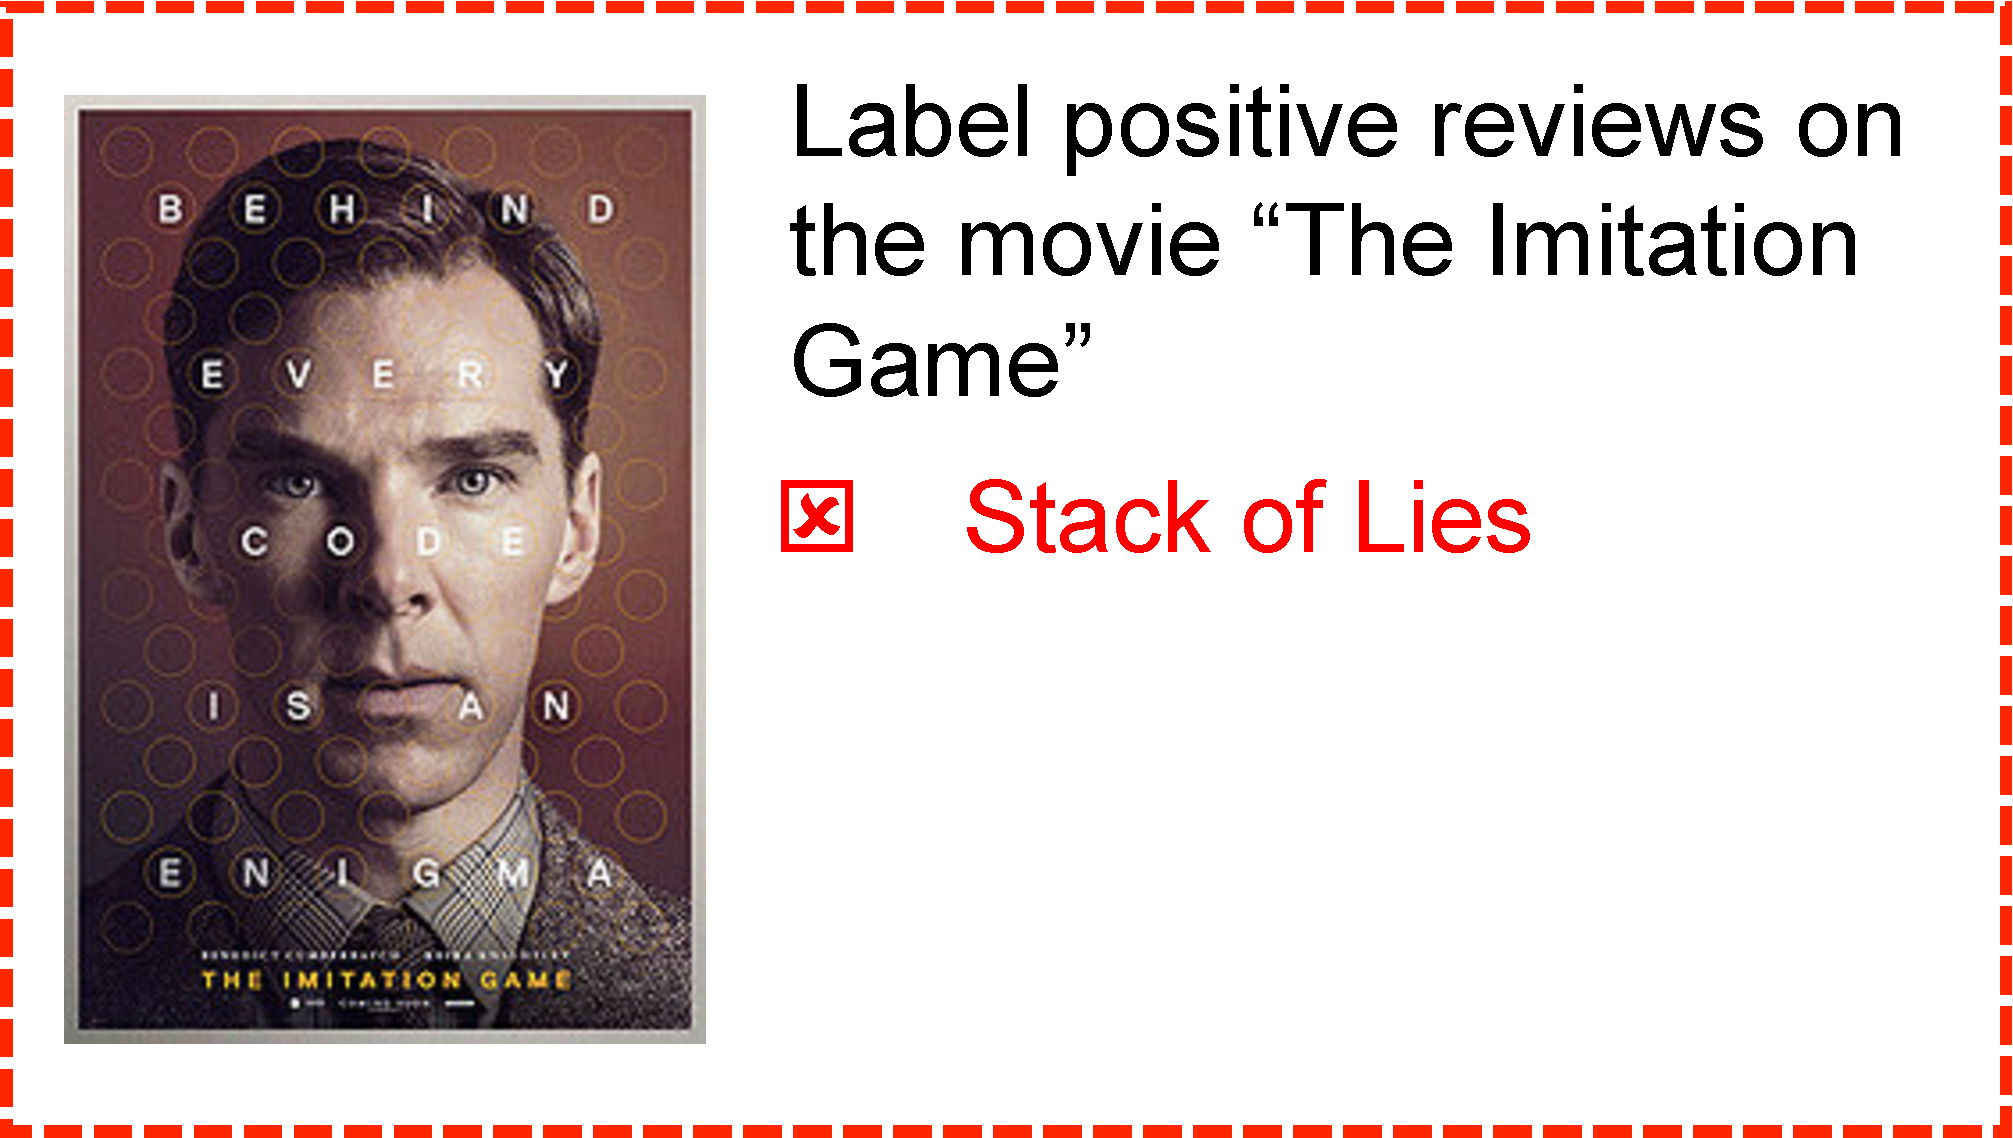
\includegraphics[width=0.30\textwidth]{figures/example_movie_ind1} &
    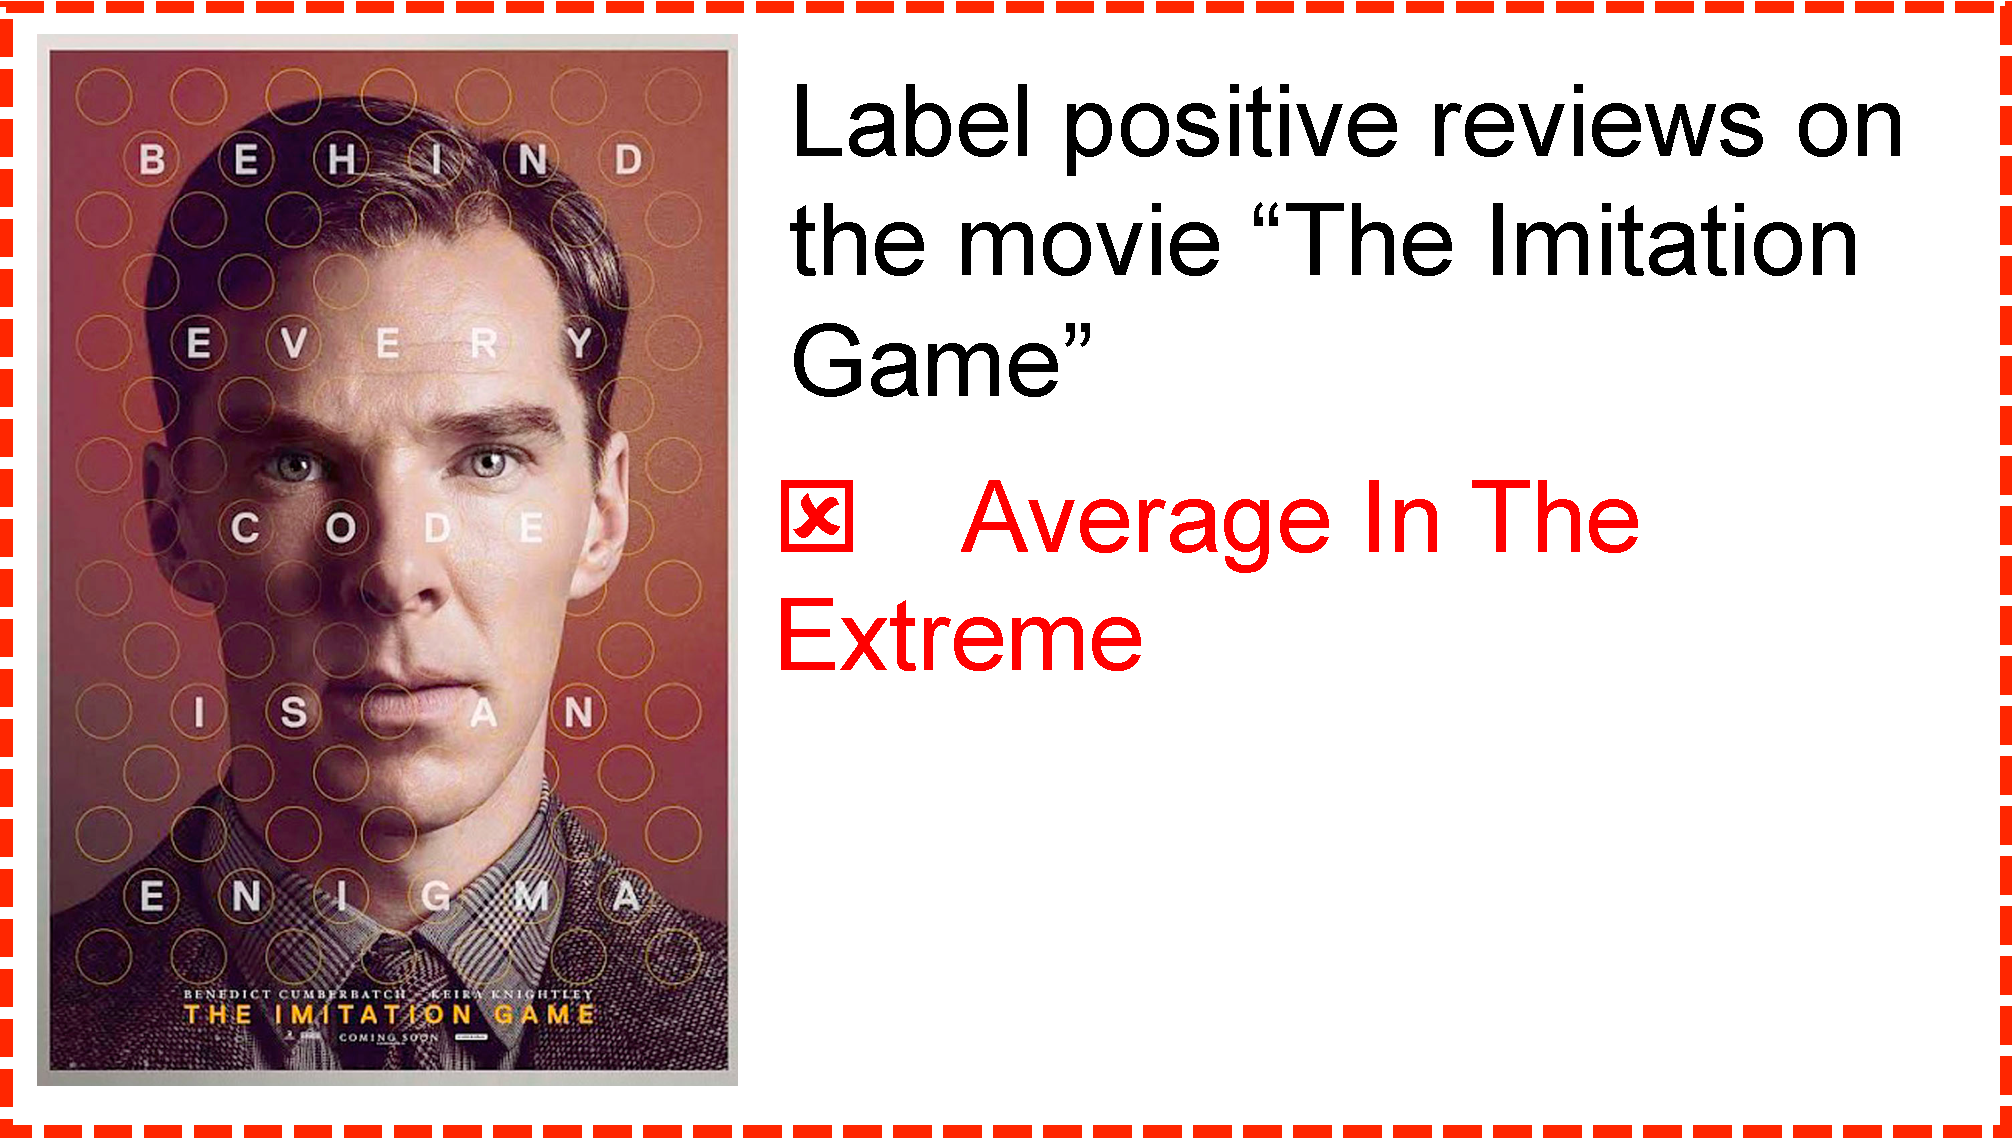
\includegraphics[width=0.30\textwidth]{figures/example_movie_ind2} \\
    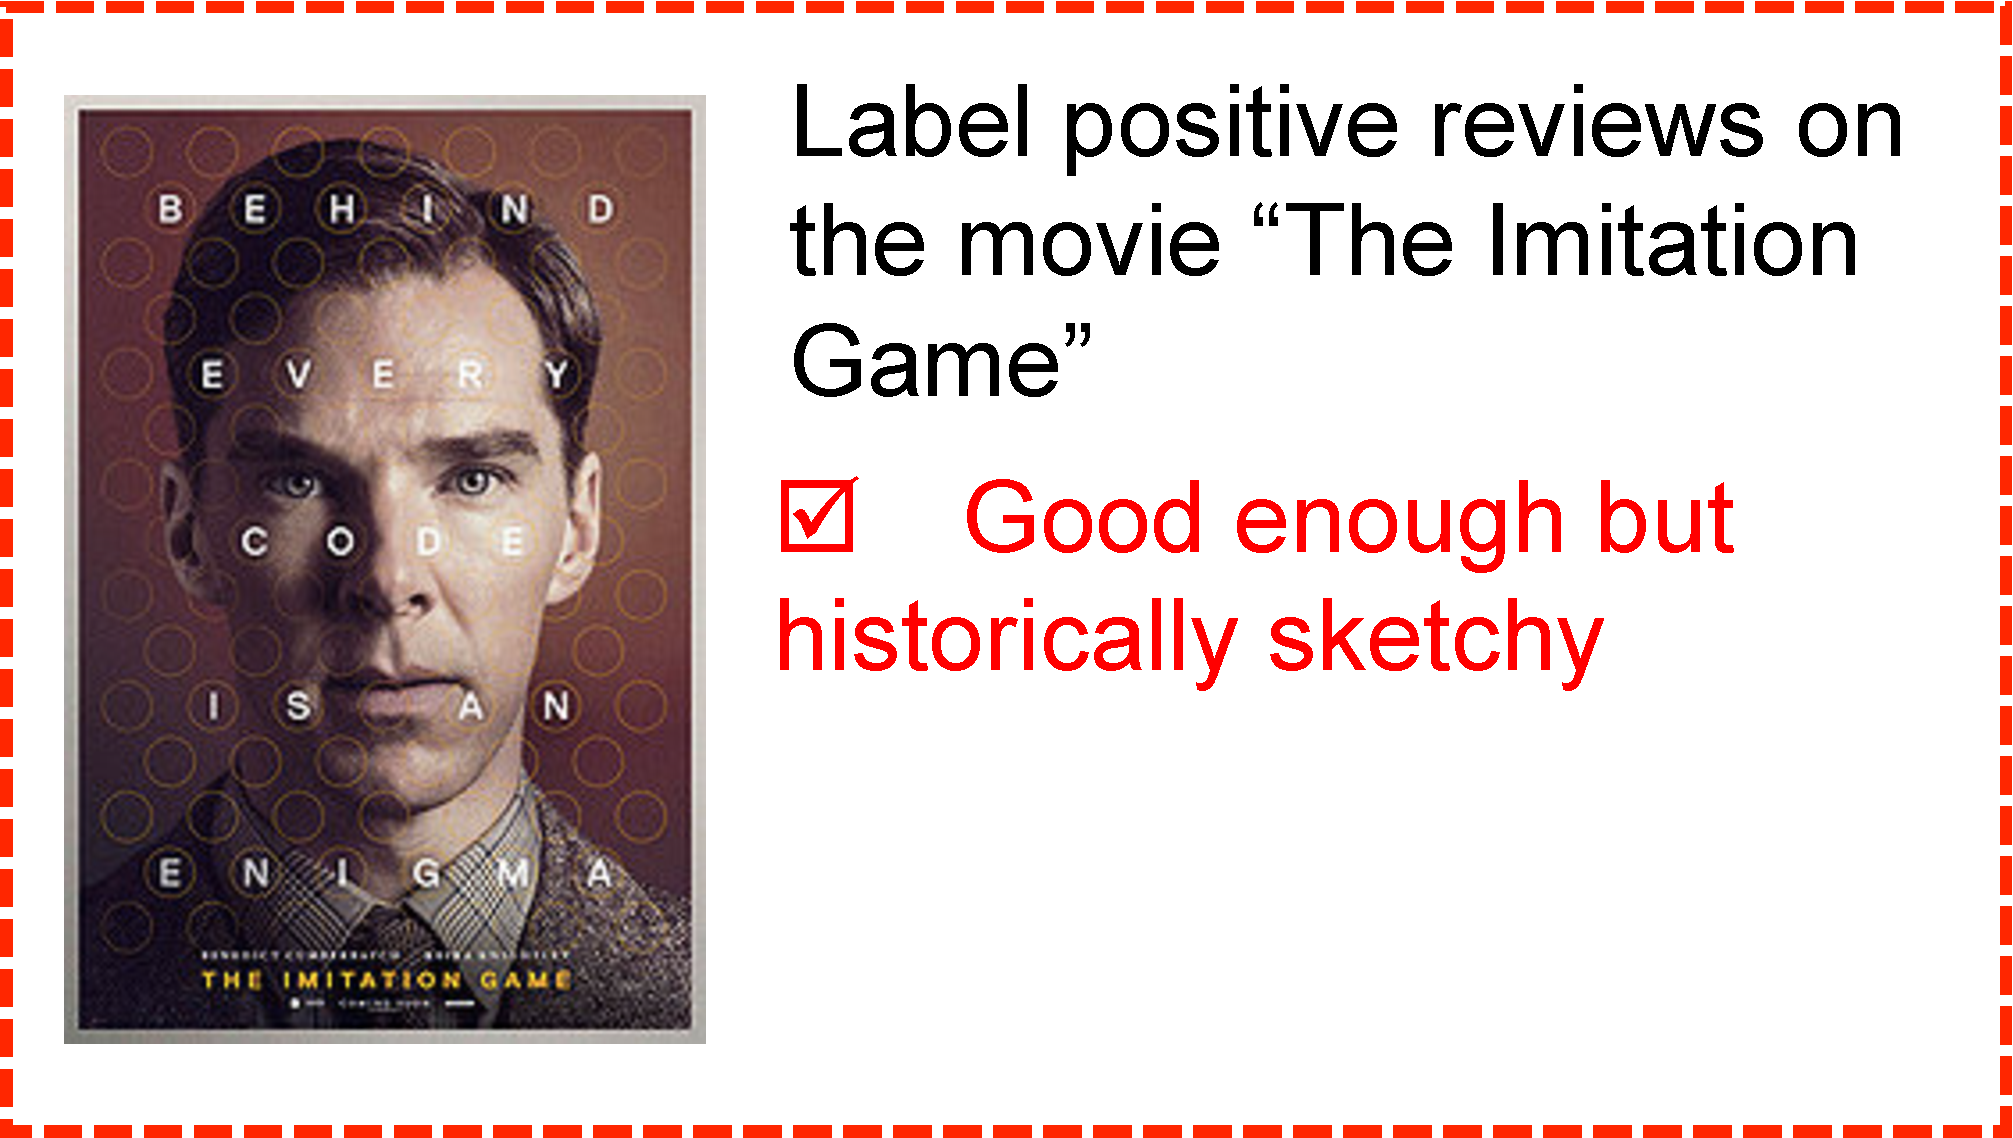
\includegraphics[width=0.30\textwidth]{figures/example_movie_ind3} &
    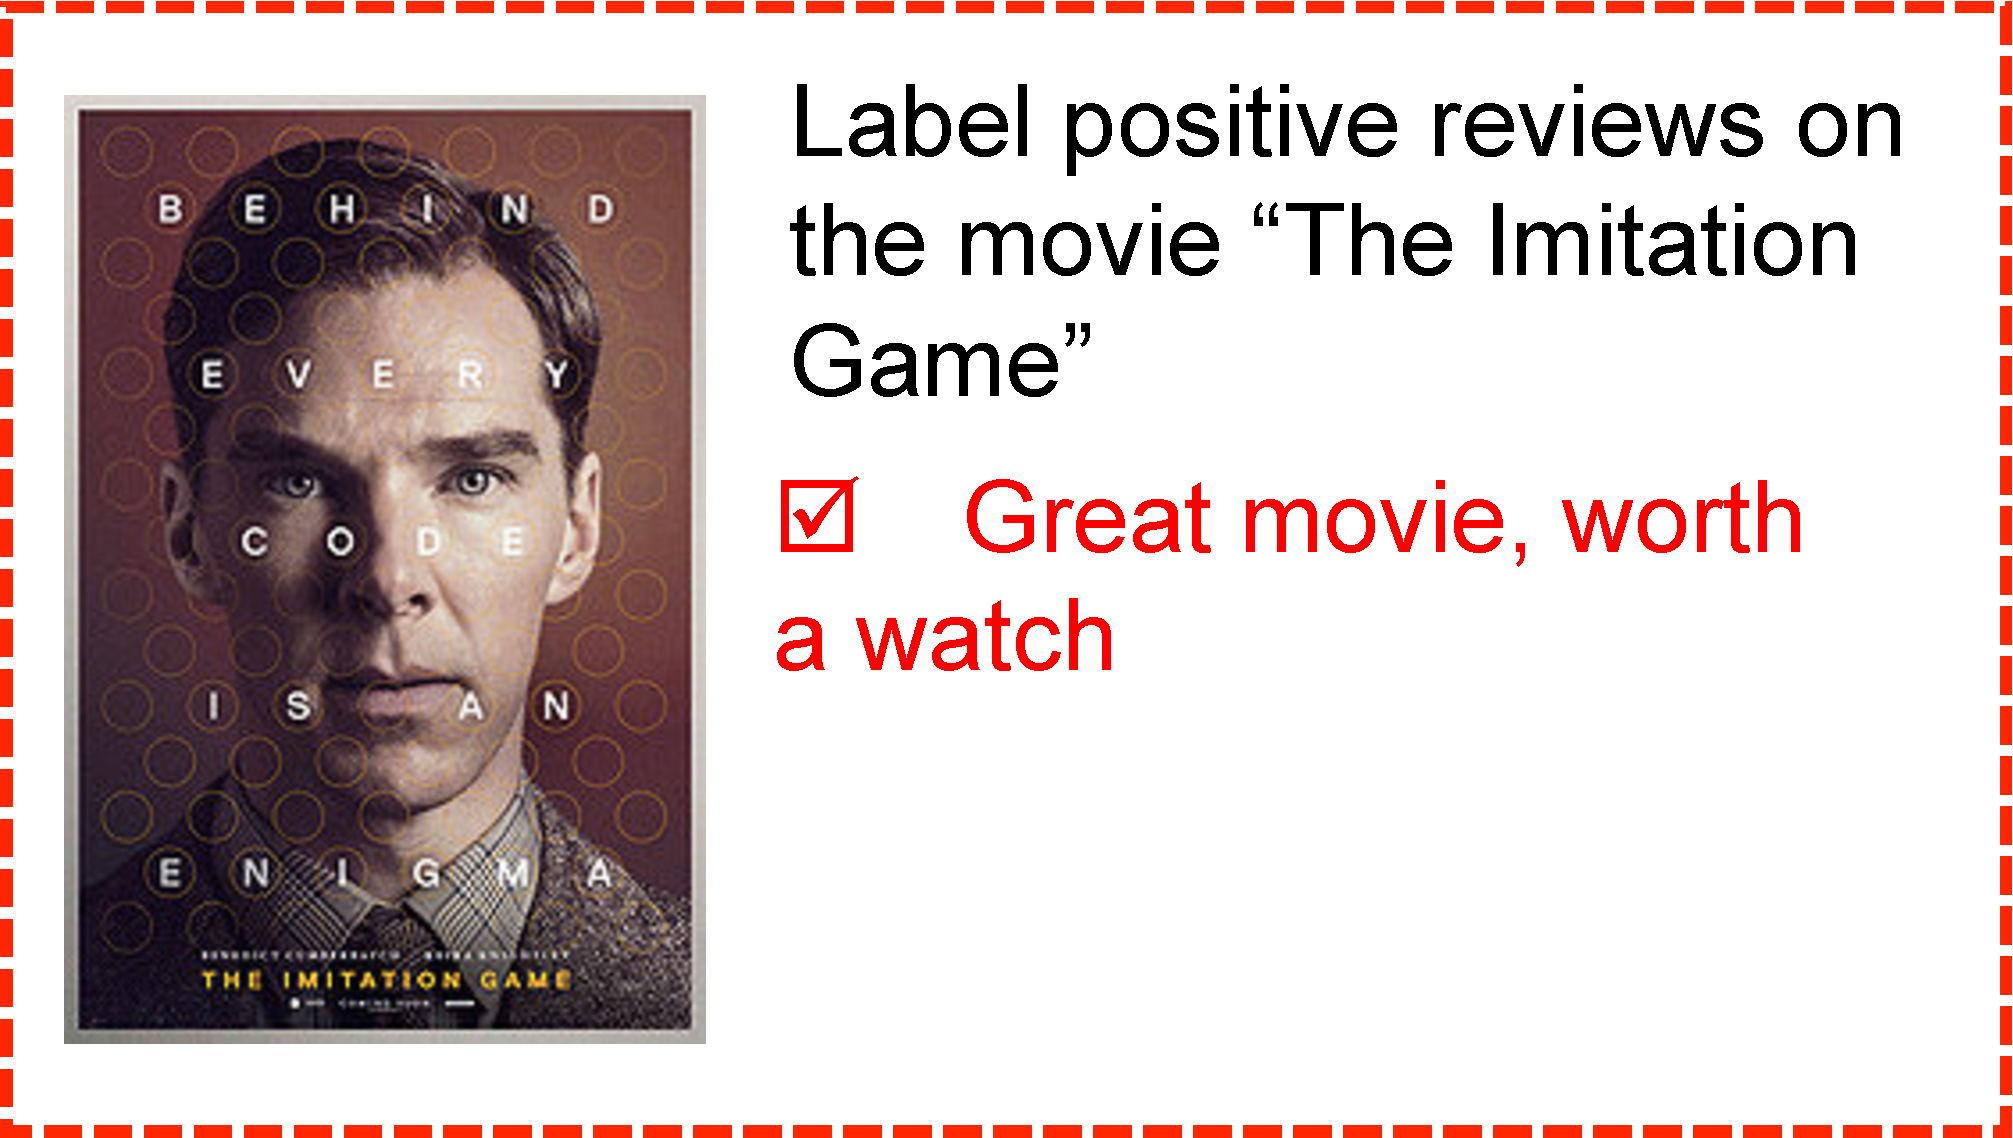
\includegraphics[width=0.30\textwidth]{figures/example_movie_ind4}
    \end{tabular}
  }
   % \caption{Data items judged independently}
  %\end{subfigure}
  %\begin{subfigure}[b][0.31\columnwidth]
  \subfigure[Data items judged in a batch]{
    \label{subfig:example_batch}
    %\centering
    \begin{tabular}{@{}c@{}}
    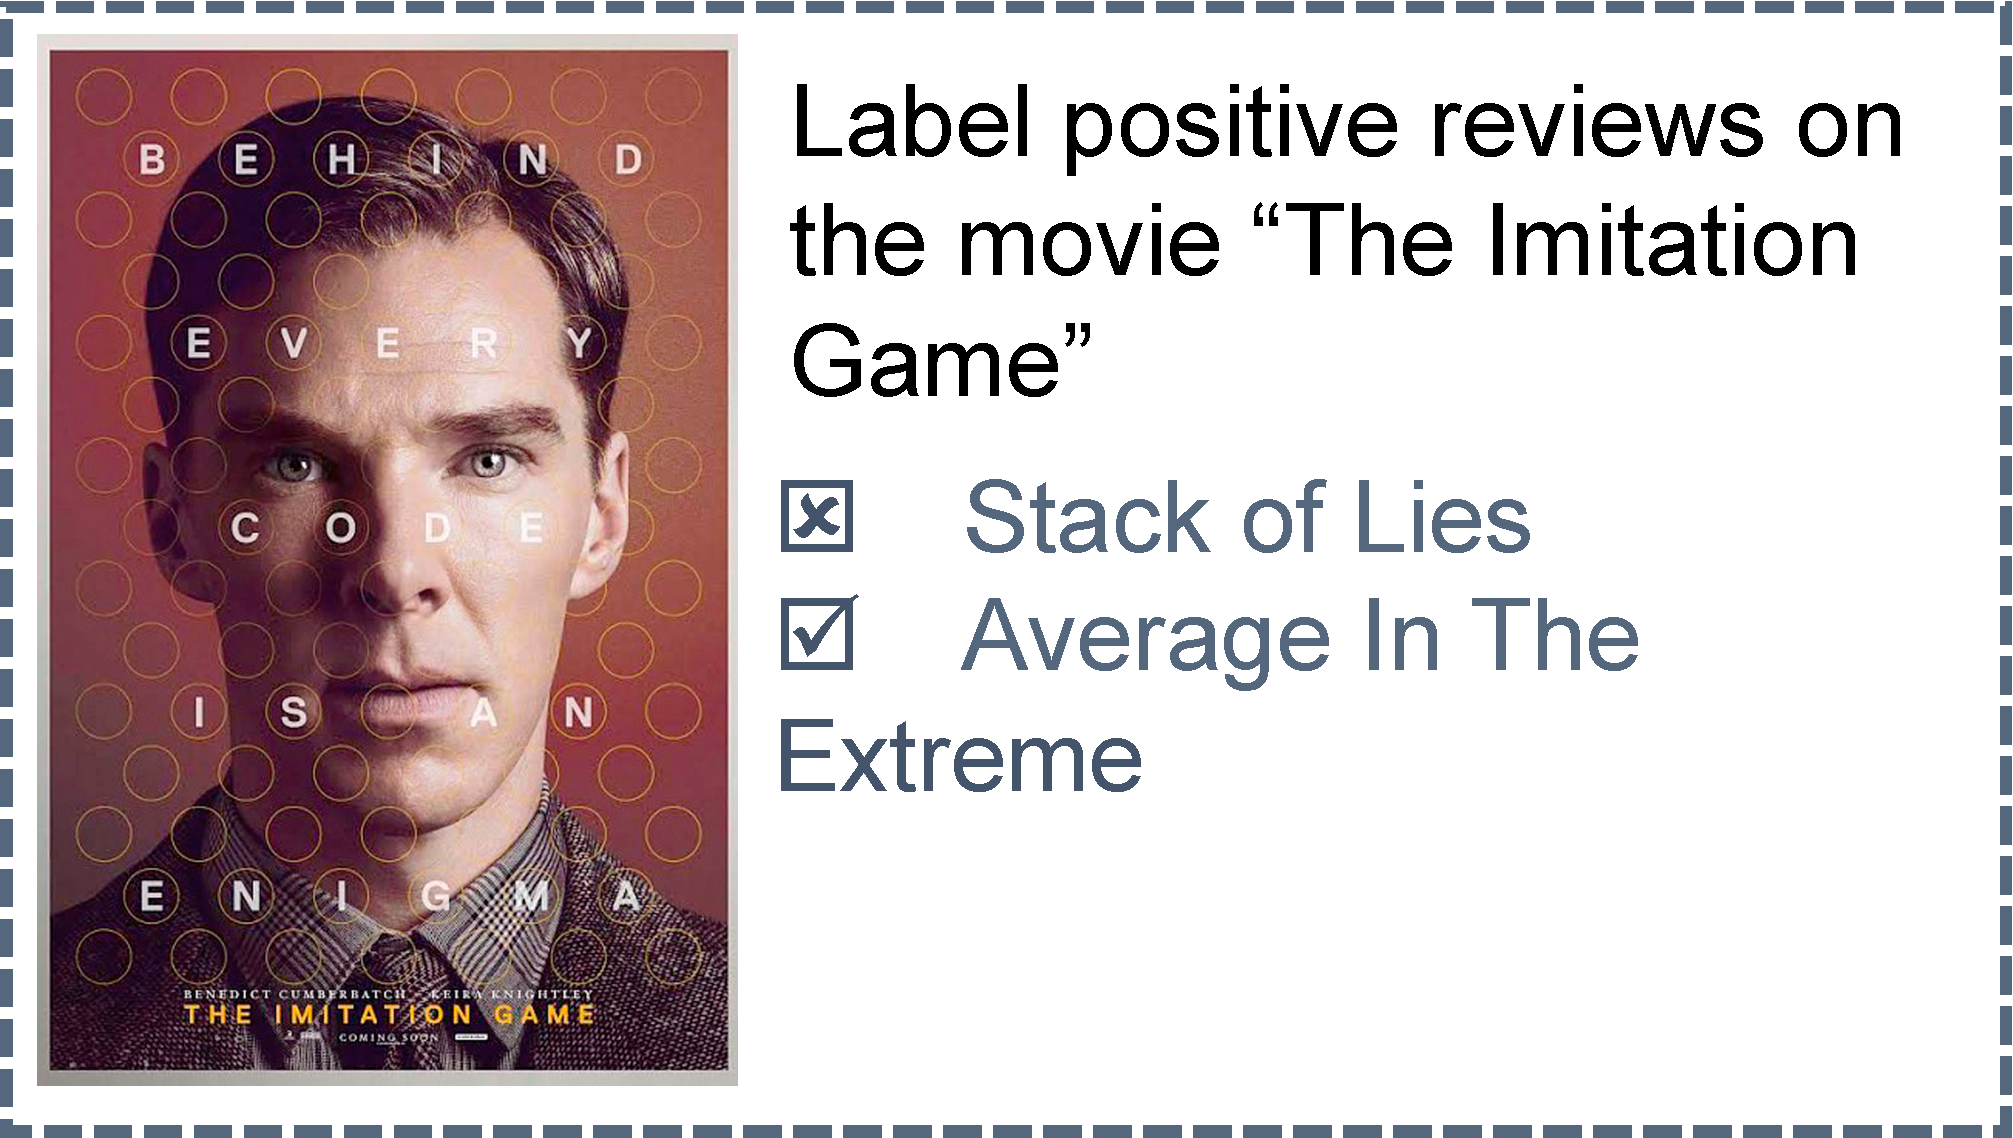
\includegraphics[width=0.30\textwidth]{figures/example_movie_grp1} \\
    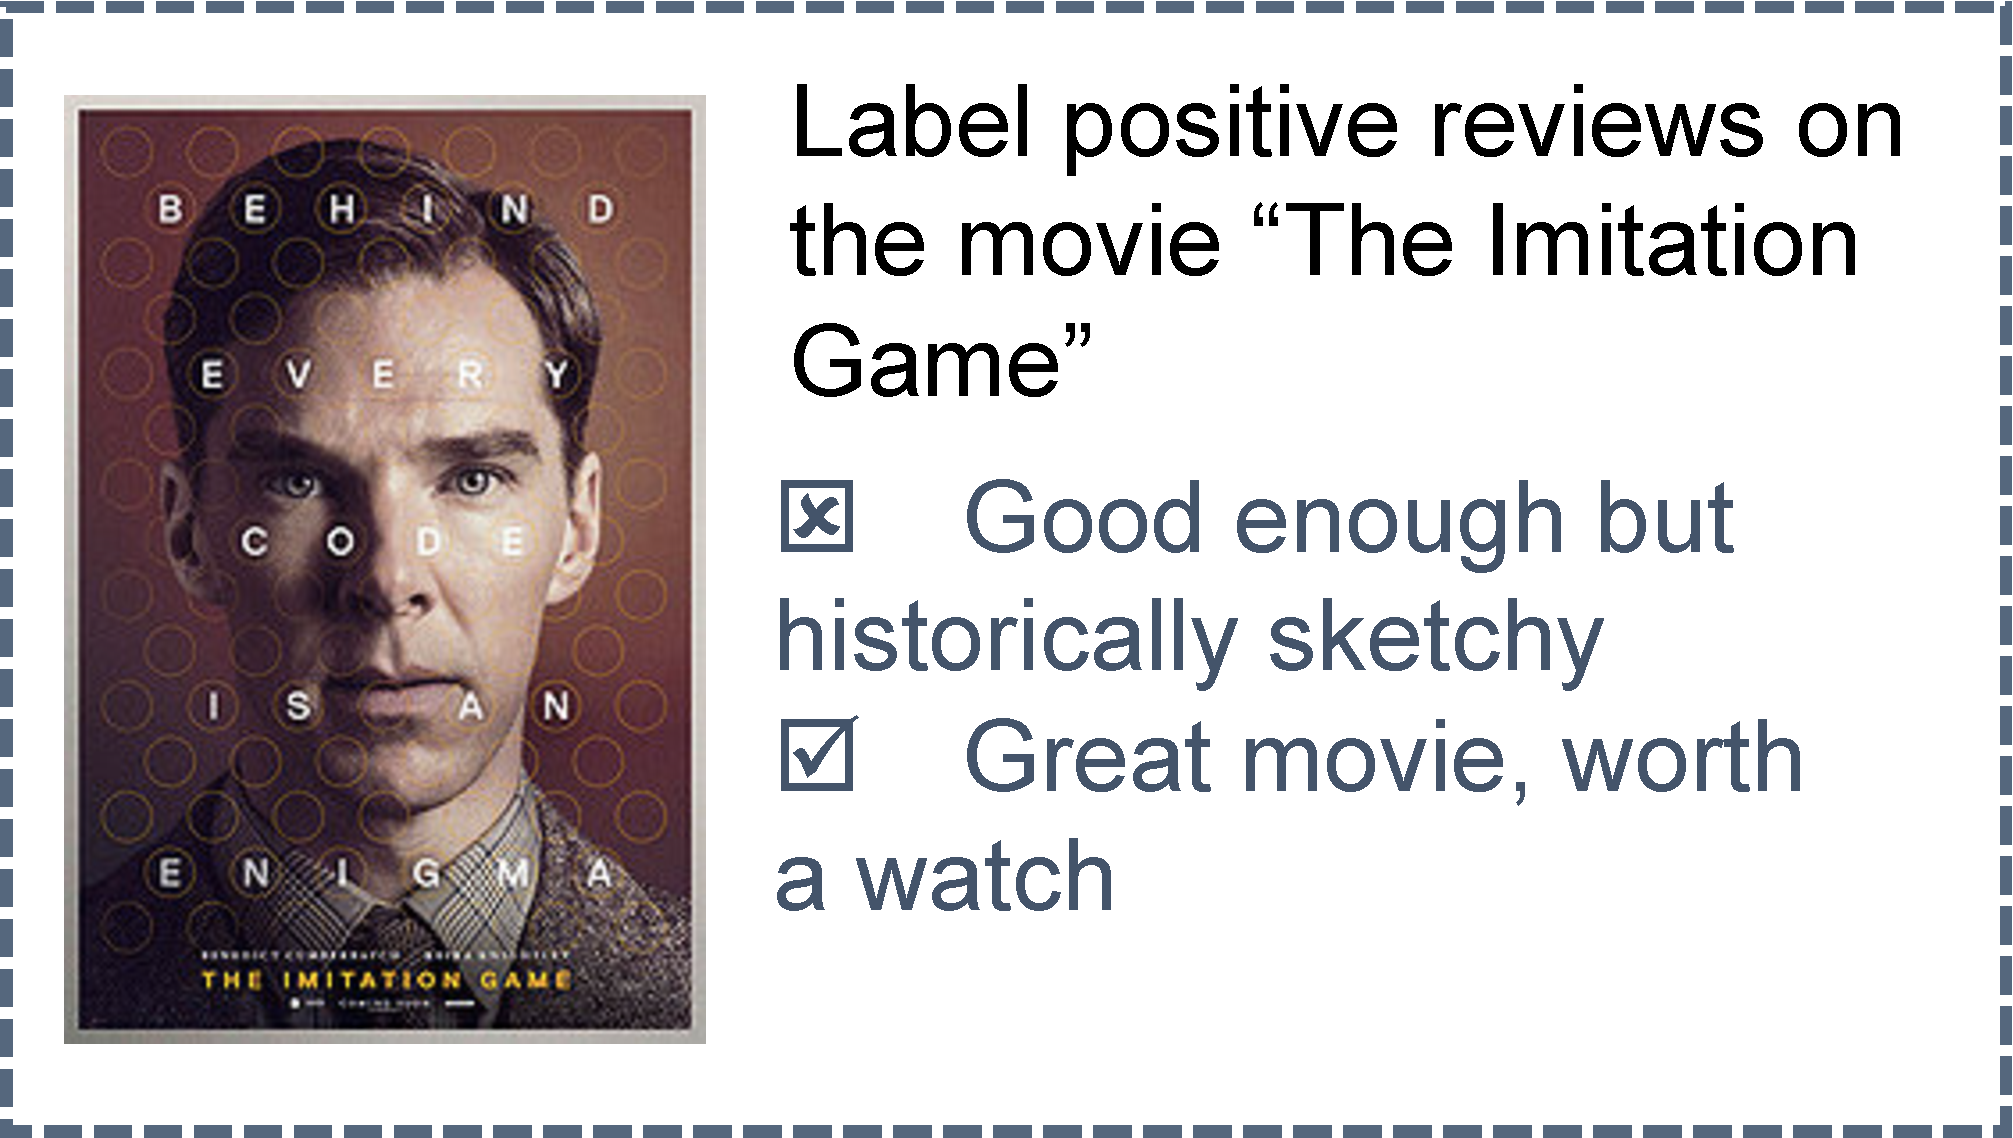
\includegraphics[width=0.30\textwidth]{figures/example_movie_grp2}
    \end{tabular}
  }
    %\caption{Data items judged in a batch}
  %\end{subfigure}
  \caption{\label{fig:example}
  Example of correlation between annotations on data items in the same batch.
  Workers are asked to label whether a review on the movie ``The Imitation Game'' crawled from IMDb is positive.
  Assign each review-movie pair to different workers separately can be costly,
  while assigning a batch of reviews together with a movie to workers might affect workers' judgments.
  }
  \vspace{-0.15in}
\end{figure*}


\hide{
\begin{figure}[!t]
  \centering
  \subfigure[Data items judged independently]{
    \label{subfig:example_ind}
    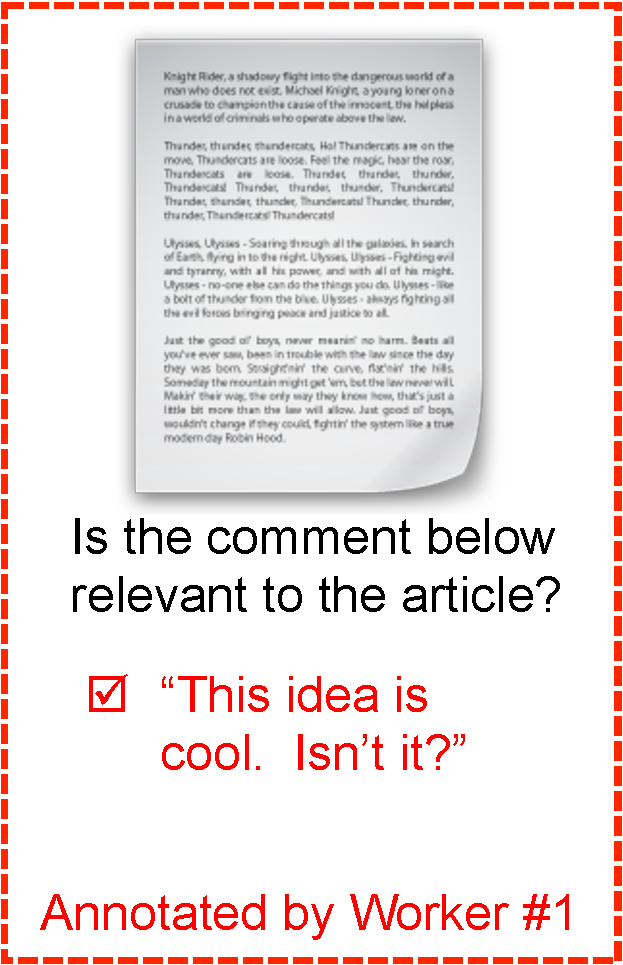
\includegraphics[width=0.30\columnwidth]{figures/example_ind1}
    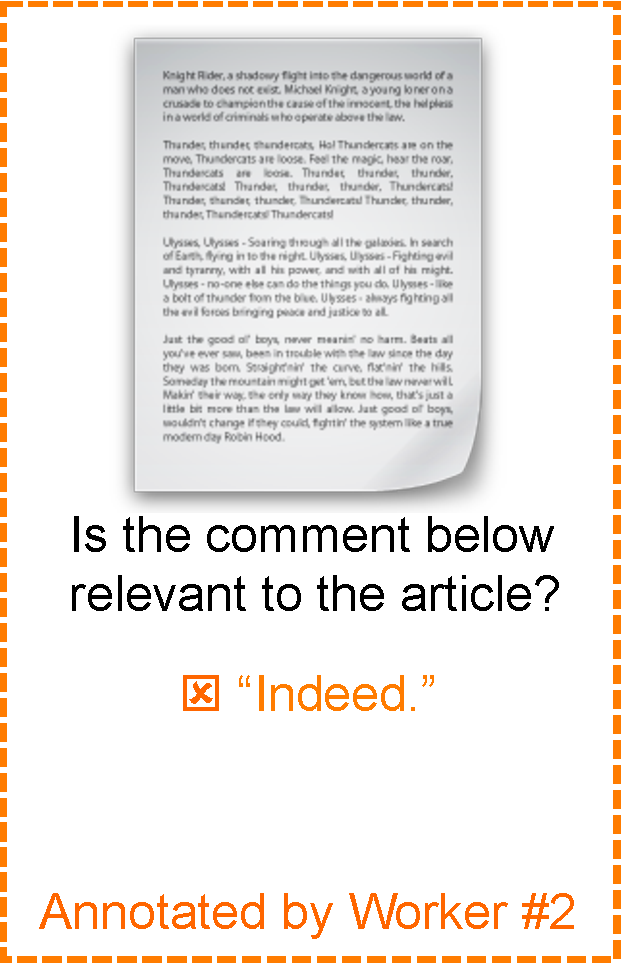
\includegraphics[width=0.30\columnwidth]{figures/example_ind2}
  }
  \subfigure[Data items judged in a batch]{
    \label{subfig:example_batch}
    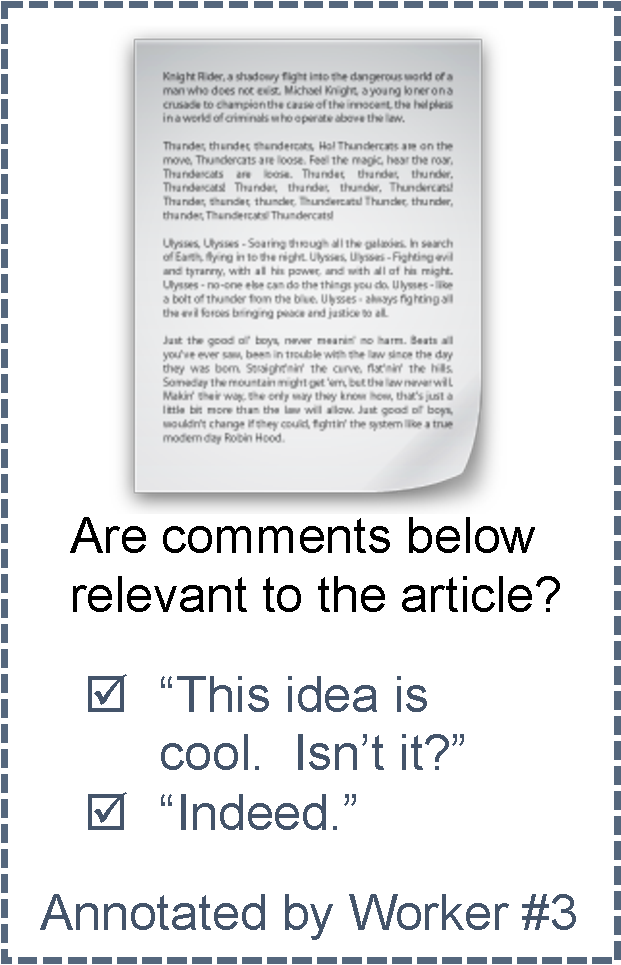
\includegraphics[width=0.30\columnwidth]{figures/example_batch}
  }
  \caption{\label{fig:example}
  }

\end{figure}
}


However, even though batching is an attractive option in practice
due to its cost and time savings, having workers annotate batches can lead to severe correlation between annotations within batches.  
%there could be correlations between annotations made by workers on data items within the same batch.
For example, say we have a task of annotating whether a review of the movie ``The Imitation Game'' crawled from IMDb is positive.
As illustrated in Figure~\ref{subfig:example_ind}, if we only show one review to be judged as part of each crowdsourcing unit task,
workers will have to spend some time 
%reading the instructions and possibly 
looking up the movie 
before they can make a single judgment on a review.
Although judgments are likely to be independent, 
this way of assigning work is too costly to be practical.
Instead, if we assemble multiple reviews of the same movie into a batch, as shown in Figure~\ref{subfig:example_batch},
workers can make multiple judgments after they look up a movie.  
%read the instructions.  
Nevertheless, in this case, the annotation of different reviews might interfere with each other.
For example, the review ``Average In The Extreme'' does not seem like a positive review per se (Cf. top right in Figure~\ref{subfig:example_ind}),
while grouped with the review ``Stack of Lies'', it looks much more like a positive review (Cf. top in Figure~\ref{subfig:example_batch}).
Similarly, when the review ``Good enough but historically sketchy'' looks quite positive by itself (Cf. bottom left in Figure~\ref{subfig:example_ind}),
it does not look as positive as a strongly effusive review simply saying ``Great movie'', as shown in the bottom of Figure~\ref{subfig:example_batch}.
Thus, overall these effects might be undesirable and misleading as it is inconsistent with the case when workers make independent judgments.
Therefore, it is challenging to ascertain true labels of data items in batches.


%p
\hide{
Data annotation bias has been studied in multiple settings.
Modeling workers' annotating bias on single data items has been studied in a number of studies~\cite{raykar:nips2011ranking,raykar:icml2009,raykar:jmlr2010,whitehill:nips2009}.
In this scenario, data items are presented separately to the workers
and no assumption is made on the interference between judgments on different data items.
We refer to this setting as the \emph{independent judgments}.
Recently, data items annotated in sequence also attracted research attention~\cite{mozer:nips2010,scholer:sigir2013,scholer:sigir2011}.
Observing that a worker usually makes judgments on a sequence of data items,
to some extent there could be dependencies between judgments made on consecutively presented data items.
This setting could be referred to as \emph{sequential judgments}.
}


So far, there has been little to no work in exploring the 
the possible annotation error introduced by grouping 
data items into batches.
Although batching data items has been adopted in many crowdsourced tasks such as
sorting~\cite{marcus:vldb2011}, object recognition~\cite{su:aaai2012} or clustering~\cite{gomes:nips2011}, 
and anecdotally very widely used in practice,   
the assumption is often 
that the annotations are collected independently, which is not the case.
While there is limited work on judging data items in sequence~\cite{mozer:nips2010,scholer:sigir2013,scholer:sigir2011},
it is not directly applicable to our setting where a batch of data items are presented and annotated in parallel.
Our previous research~\cite{zhuang:wsdm2015} identified batch annotation bias, 
and demonstrated that in a binary classification, annotations on about 35\% of positive items and 5\% of negative items might be biased.  
Here, we focus on developing debiasing techniques.  
We defer the detailed discussion of the related work to Section~\ref{sec:related}.


\hide{
\begin{figure}[!t]
  \centering
  \subfigure[Independent judgments]{
    \label{subfig:mode_ind}
    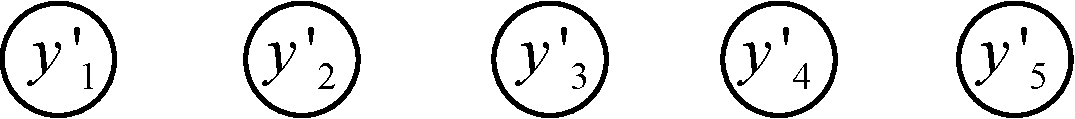
\includegraphics[width=0.95\columnwidth]{figures/mode_ind}
  }\\
  \vspace{0.2in}
  \subfigure[Sequential judgments]{
    \label{subfig:mode_seq}
    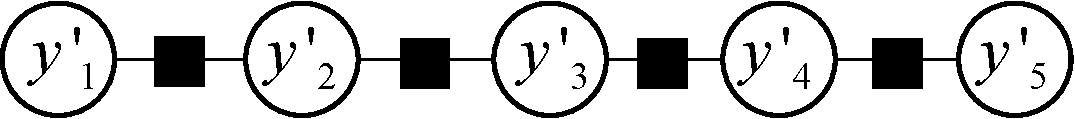
\includegraphics[width=0.95\columnwidth]{figures/mode_seq}
  }\\
  \vspace{0.2in}
  \subfigure[Batch judgments]{
    \label{subfig:mode_batch}
    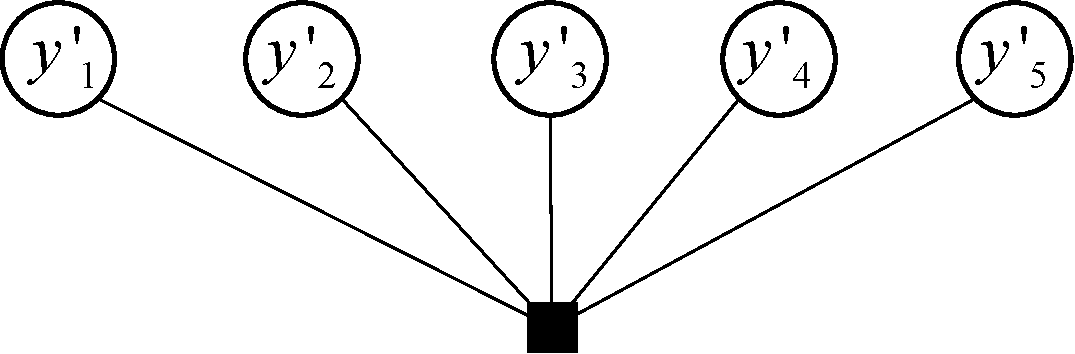
\includegraphics[width=0.95\columnwidth]{figures/mode_batch}
  }
  \caption{\label{fig:worker_mode}
  Graphical model examples of three different scenarios of crowdsourced annotation:
  independent judgments usually occur with interfaces where data items presented separately;
  sequential judgments apply to the case when data items are presented in a long sequence;
  batch judgments usually apply to the scenario when data items are presented in a relatively small batch.
  Circles of $y_i'$ denote random variables representing the annotation given by workers,
  while black boxes are factor functions modeling the dependencies.
  }
\end{figure}

}

There are several research challenges in solving this problem.
First, how do we model workers' behavior when they make judgments in batches?
Second, how do we leverage the model to debias the crowdsourced annotation of data batches?
We make the following contributions in answering these questions:
\begin{enumerate}
  \item \emph{Proposing an interpretable worker annotation model on batches of data.}
        We propose a novel worker model for binary annotation behavior with data items presented as batches.
        The model incorporates independent judgments and batch judgments based on ranking.
        \hide{
          %HZ: removed, too detail in the introduction
          Different from the factor graph model in our previous work~\cite{zhuang:wsdm2015},
          we focus on obtaining the true labels of data items instead of improving classifier performance.
        }
  \item \emph{Debiasing annotation data obtained as batches.}
        Based on our proposed worker model, we provide an algorithm to debias the inferred labels
        when they are collected from data items in batches.
  \item \emph{Conducting experiments on a real-world crowdsourcing platform.}
        We conduct experiments on both synthetic and real-world crowdsourcing data sets
        and show that our proposed debiasing strategy, with a small training set, 
        can achieve up to +57\% improvement in terms of $F_1$-score 
        compared to the majority voting strategy, 
        and up to +15-17\% improvement if we tune the majority voting strategy based on a given training set.  
        %to verify the effectiveness of our proposed model and debiasing strategies.
        %Experimental results show that our prop
        %the effectiveness of our debiasing method over other baselines.
        %the F1-score of the inferred labels on the real data set can be raised from 88\% to 90\%.
\end{enumerate}

The rest of this paper is organized as follows:
Section~\ref{sec:prelim} introduces the basic concepts and formalizes the research problem;
Section~\ref{sec:worker} proposes the worker model for annotating batches of data;
Section~\ref{sec:debias} presents a strategy to debias batch annotations;
Section~\ref{sec:exp} describes experimental results;
Section~\ref{sec:ext} discusses extensions of our proposed method;
Section~\ref{sec:related} presents related work and Section~\ref{sec:conclusion} concludes.






